\documentclass[10pt]{article}

\usepackage[T1]{fontenc}
\usepackage[margin=1in]{geometry}
\usepackage{setspace}
\usepackage{hyperref}
\usepackage{longtable}
\usepackage{titlesec}
\usepackage{listings}
\usepackage{xcolor}
\usepackage{booktabs}
\usepackage{enumitem}
\usepackage{microtype}
\usepackage{cite}
\usepackage{graphicx}
\usepackage{float}
\setlist{noitemsep, topsep=3pt, partopsep=0pt}

\setstretch{1.15}

\titleformat{\section}{\normalfont\Large\bfseries}{\thesection}{1em}{}
\titleformat{\subsection}{\normalfont\large\bfseries}{\thesubsection}{1em}{}
\titleformat{\subsubsection}{\normalfont\normalsize\bfseries}{\thesubsubsection}{1em}{}

\lstset{
  basicstyle=\ttfamily\small,
  breaklines=true,
  frame=single,
  backgroundcolor=\color{gray!8},
  rulecolor=\color{gray!40},
}

\title{PyCodeKG: Deterministic Code Navigation via Knowledge Graphs,
Semantic Indexing, and Grounded Context Packing}

\author{Eric G. Suchanek, PhD\\
Flux-Frontiers, Liberty Township OH\\[4pt]
\small\url{https://github.com/Flux-Frontiers/pycode\_kg}}
\date{}

\begin{document}

\maketitle

\begin{abstract}
PyCodeKG is a \emph{knowledge compiler} for Python codebases. Rather than
indexing source text for retrieval, it transforms source code into a
progressively enriched knowledge graph through five deterministic, ontology-driven
enrichment phases: structural extraction, call-graph construction, data-flow
analysis, cross-module symbol resolution, and semantic indexing. Each phase adds
a semantic layer that its predecessor cannot express; the ordering is determined
by the semantic dependencies of the Python ontology, not by implementation
convenience. The result is a compiled knowledge artifact---richer than any
single-pass extraction could yield---that did not exist in the source and cannot
be recovered by reading any individual file.

Structural relationships---definitions, calls, imports, and inheritance---and
data-flow relationships---variable reads, writes, and attribute accesses---are
extracted directly from the Python abstract syntax tree and stored in SQLite,
which is the authoritative record. A vector index over the same nodes, built
with sentence-transformer embeddings and stored in LanceDB, provides
natural-language entry points into the structurally complete graph without
replacing or overriding it.

The system is organized into four core layers---a pure AST extractor
(\texttt{CodeGraph}), a relational graph store (\texttt{GraphStore}), a semantic
vector index (\texttt{SemanticIndex}), and an orchestrator (\texttt{PyCodeKG})---plus a
\texttt{KGModule} extensibility SDK that abstracts the full build/query/pack pipeline
behind a two-method interface so the infrastructure can be reused for any knowledge
graph domain. A built-in CLI exposes the full pipeline directly; adapter layers (MCP server,
Streamlit visualizer, 3-D PyVista graph) make the same capabilities available to
IDE-integrated AI agents and interactive exploration workflows.

PyCodeKG is independently useful without a language model. When coupled with a
downstream language model for synthesis, it constitutes a form of
knowledge-graph-augmented generation (KG-RAG). It differs fundamentally
from the LLM-constructed graph approach of Microsoft GraphRAG~\cite{edge2024graphrag}:
the knowledge graph is \emph{compiled} from formal syntax rather than \emph{inferred}
from natural language, making it structurally correct by construction rather than
probabilistically approximate. We term this \emph{Structural KG-RAG}.
\end{abstract}

\section{Introduction}

As Python systems grow, answering basic architectural questions becomes surprisingly
hard. Where is this configuration value actually set? Which functions participate in
the connection lifecycle? Where is this service called, and under what conditions?
Text search finds strings; IDE symbol lookup finds definitions. Neither tells you
much about the shape of the system.

Large language models offer a different kind of help---they can reason about code
semantically---but they are not grounded in the source tree. Without a structural
substrate, they may confuse function signatures, misrepresent call relationships,
or describe code that does not exist. The problem is not intelligence; it is the
absence of a reliable structural anchor.

PyCodeKG addresses this by building that substrate first. The Python AST is parsed
deterministically, producing a graph of nodes (modules, classes, functions, methods)
and typed edges (CONTAINS, CALLS, IMPORTS, INHERITS). That graph is stored in
SQLite, which is the authoritative record. Semantic embeddings are then built on top
of it---not instead of it---so that natural-language queries can find relevant
entry points without inventing structure that is not there.

A \emph{snippet}, as used throughout this paper, is a source-grounded code excerpt
extracted at a verified file path and exact line span, annotated with node metadata,
and suitable for direct LLM consumption.

This approach is deliberately inverted relative to systems such as Microsoft
GraphRAG~\cite{edge2024graphrag}, which use an LLM to \emph{construct} a knowledge
graph from unstructured text. In PyCodeKG, the LLM has no role in graph construction:
the graph is extracted from formal syntax, and the LLM's role is to \emph{reason
against} the resulting source-grounded context. Section~\ref{sec:comparison} develops
this contrast in detail.

\section{Design Principles}

Six principles govern the design:

\begin{enumerate}
\item \textbf{Structure is authoritative.}
The AST-derived graph is the source of truth. Embeddings are derived from it and
can be discarded and rebuilt at any time without loss.

\item \textbf{Semantics accelerate, never decide.}
Vector search identifies candidate entry points. Graph traversal determines what
is actually returned. The two phases are explicit and separable.

\item \textbf{Everything is traceable.}
Every node carries a file path and line span. Every edge may carry evidence---a
line number and expression text from the call site. Nothing is inferred without
a source location.

\item \textbf{Determinism over heuristics.}
Identical input produces identical output. There are no probabilistic components
in the structural layer.

\item \textbf{Composable artifacts.}
SQLite, LanceDB, Markdown, and JSON are independent outputs. Any downstream
consumer---a human, an agent, a CI pipeline---can use whichever format suits it.

\item \textbf{Compilation over retrieval.}
PyCodeKG does not retrieve from an existing corpus. It \emph{compiles} a new
knowledge artifact from source through a sequence of enrichment passes, each
adding a semantic layer that the previous pass could not express. The enrichment
sequence is determined by the semantic dependencies of the Python ontology:
structural containment must be established before call relationships can be
recorded; call stubs must exist before cross-module resolution can proceed; the
complete structural record must be stable before semantic embeddings can be
meaningfully derived. The resulting graph encodes more about the codebase---and
more reliably---than any single-pass extraction could yield.
\end{enumerate}

\section{Architecture}

\begin{figure}[H]
\centering
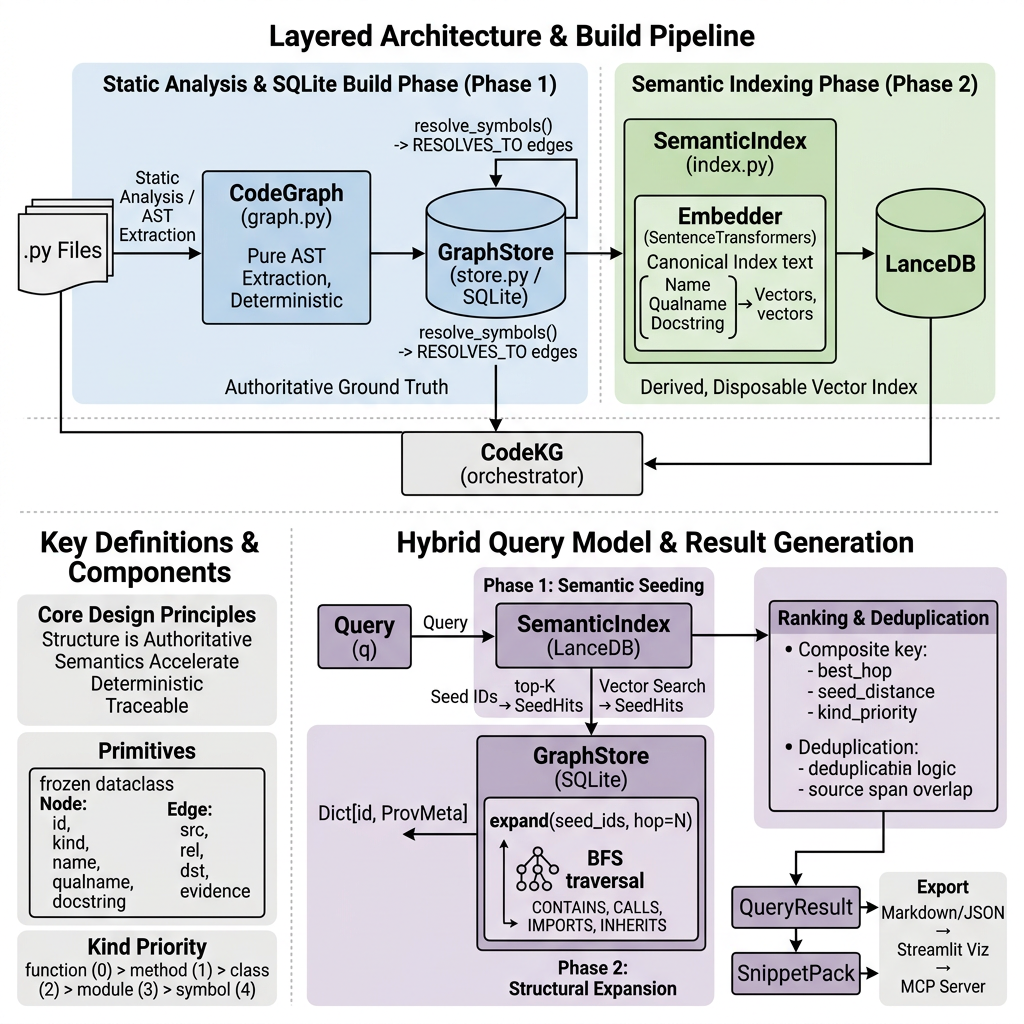
\includegraphics[width=0.85\linewidth]{../assets/codeKG_arch_banana.png}
\caption{PyCodeKG layered architecture and build pipeline. Phase~1 (left) performs
static AST extraction into SQLite; Phase~2 (centre) builds the LanceDB semantic
index; the hybrid query model (right) seeds from the vector index and expands
structurally through the graph to produce ranked, source-grounded results.}
\label{fig:architecture}
\end{figure}

The implementation is organized into six layers plus a companion data-flow
extraction module. Each layer has a single responsibility and depends only on
layers below it.

\subsection{Layer 1 --- Primitives (\texttt{pycodekg.py})}

Two frozen dataclasses and one extraction function form the foundation.

\textbf{\texttt{Node}} carries: \texttt{id} (stable, deterministic), \texttt{kind},
\texttt{name}, \texttt{qualname}, \texttt{module\_path}, \texttt{lineno},
\texttt{end\_lineno}, and \texttt{docstring}.

\textbf{\texttt{Edge}} carries: \texttt{src}, \texttt{rel}, \texttt{dst}, and
optional \texttt{evidence} (a JSON object, typically \texttt{\{lineno, expr\}}).

\textbf{\texttt{extract\_repo(repo\_root)}} walks all \texttt{.py} files and runs
two deterministic AST passes. Pass~1 extracts definitions and emits
\texttt{CONTAINS}, \texttt{IMPORTS}, and \texttt{INHERITS} edges. Pass~2 extracts
the call graph, emitting \texttt{CALLS} edges with call-site evidence. Unresolved
call targets become \texttt{sym:} symbol nodes.

Supported node kinds: \texttt{module}, \texttt{class}, \texttt{function},
\texttt{method}, \texttt{symbol}.
Structural edge relations: \texttt{CONTAINS}, \texttt{CALLS}, \texttt{IMPORTS},
\texttt{INHERITS}. A fifth structural relation, \texttt{RESOLVES\_TO}, is added
in a post-build step by \texttt{GraphStore.resolve\_symbols()} (see
Section~\ref{sec:graphstore}).
Data-flow edge relations: \texttt{READS}, \texttt{WRITES}, \texttt{ATTR\_ACCESS}
(emitted by \texttt{PyCodeKGVisitor}; see Section~\ref{sec:visitor}).

\subsection{Data-Flow Visitor (\texttt{visitor.py})}
\label{sec:visitor}

\texttt{PyCodeKGVisitor} extends \texttt{ast.NodeVisitor} to capture intra-function
data-flow relationships that the structural pass in \texttt{pycodekg.py} does not
record. Where \texttt{extract\_repo} answers \emph{what exists and how it is
called}, \texttt{PyCodeKGVisitor} answers \emph{what each function reads and writes}.

The visitor maintains a scope stack and a per-scope variable registry. On entering
a function or method, all parameter names---positional, keyword-only, variadic, and
keyword-variadic---are seeded into the local variable set. Default argument
expressions are attributed to the \emph{enclosing} scope rather than the function
being defined, matching Python's evaluation semantics. \texttt{async def} nodes are
handled identically to \texttt{def}.

Three data-flow edge types are emitted:

\begin{itemize}
\item \textbf{\texttt{READS}} --- emitted for every variable name loaded in an
assignment right-hand side, call argument, keyword argument value, or default
expression. Records where data enters a computation.
\item \textbf{\texttt{WRITES}} --- emitted for every assignment target. Records
where a variable is defined or updated within a scope.
\item \textbf{\texttt{ATTR\_ACCESS}} --- emitted when a named object is accessed
via attribute notation (\texttt{obj.attr}), connecting the object's variable node
to a node representing the accessed attribute within the same scope.
\end{itemize}

All edges carry a source line number extracted from the originating AST node.
The visitor is invoked per file and produces nodes and edges compatible with the
\texttt{GraphStore} schema via \texttt{finalize()}.

\subsection{Layer 2 --- \texttt{CodeGraph} (\texttt{graph.py})}

\texttt{CodeGraph} wraps \texttt{extract\_repo} with lazy caching. The
\texttt{.nodes} and \texttt{.edges} properties trigger extraction on first access;
\texttt{extract(force=True)} re-runs from scratch. No I/O, no persistence, no
embeddings---pure AST extraction with a clean object interface.

\subsection{Layer 3 --- \texttt{GraphStore} (\texttt{store.py})}
\label{sec:graphstore}

\texttt{GraphStore} manages the SQLite \texttt{nodes} and \texttt{edges} tables and
provides the traversal primitives used by the query layer.

\begin{itemize}
\item \texttt{write(nodes, edges, wipe=False)} --- persist a complete graph via
upsert.
\item \texttt{node(id)} --- fetch a single node dict by stable identifier.
\item \texttt{query\_nodes(kinds=None, module=None)} --- filtered node list.
\item \texttt{edges\_within(node\_ids)} --- edges with both endpoints in the given
set.
\item \texttt{expand(seed\_ids, hop=1, rels=\ldots)} --- BFS expansion returning
\texttt{Dict[str, ProvMeta]}.
\item \texttt{resolve\_symbols()} --- post-build step that name-matches every
\texttt{sym:} stub against all first-party definitions and writes
\texttt{RESOLVES\_TO} edges. Idempotent; called automatically after each build.
\item \texttt{callers\_of(node\_id, rel="CALLS")} --- two-phase reverse lookup:
(1)~direct incoming \texttt{rel} edges and (2)~callers through \texttt{sym:} stubs
via \texttt{RESOLVES\_TO}. Returns deduplicated caller node dicts.
\item \texttt{stats()} --- node and edge counts by kind and relation.
\end{itemize}

\texttt{ProvMeta} records \texttt{best\_hop} (minimum hop distance from any seed)
and \texttt{via\_seed} (the originating seed node ID). This provenance is used
downstream for ranking.

\subsection{Layer 4 --- \texttt{SemanticIndex} (\texttt{index.py})}

\texttt{SemanticIndex} reads nodes from a \texttt{GraphStore}, constructs a
canonical text document for each (name plus docstring), embeds them in batches
using a pluggable \texttt{Embedder} backend, and stores the vectors in LanceDB.
The \texttt{search(query, k)} method returns a ranked list of \texttt{SeedHit}
objects carrying node ID, embedding distance, and rank.

The \texttt{Embedder} abstract class defines \texttt{embed\_texts(texts)} and
\texttt{embed\_query(query)}. The default implementation,
\texttt{SentenceTransformerEmbedder}, uses \texttt{BAAI/bge-small-en-v1.5}
via the \texttt{sentence-transformers} library (384-dimensional embeddings).
The model is overridable via the \texttt{CODEKG\_MODEL} environment variable or
the \texttt{--model} CLI flag.

The vector index is derived from SQLite and is fully disposable. Deleting and
rebuilding it does not affect the structural record.

\subsection{Layer 5 --- \texttt{KGModule} SDK (\texttt{module/})}

\texttt{KGModule} (\texttt{module/base.py}) is an abstract base class that packages
the complete build/query/pack/snapshot pipeline so domain authors can reuse it
for any knowledge graph domain by implementing exactly two abstract methods:
\texttt{make\_extractor()} and \texttt{kind()}.  All generic infrastructure---SQLite
persistence, LanceDB indexing, hybrid query, snippet packing, symbol resolution,
and snapshot management---is inherited rather than reimplemented.

\texttt{KGExtractor} (\texttt{module/extractor.py}) defines the domain-specific
extraction protocol: \texttt{node\_kinds()}, \texttt{edge\_kinds()}, and an
\texttt{extract()} generator that yields \texttt{NodeSpec} and \texttt{EdgeSpec}
objects.  \texttt{NodeSpec}/\texttt{EdgeSpec} are thin, v0-locked intermediates that
map cleanly onto the \texttt{Node}/\texttt{Edge} primitives.

\texttt{PyCodeKGExtractor} is the Python-AST-backed implementation used by
\texttt{PyCodeKG}.  Any other knowledge graph domain (\emph{e.g.}, TypeScript,
documentation corpora, metabolic pathways) can reuse the full infrastructure by
subclassing \texttt{KGModule} and providing its own \texttt{KGExtractor}.

\subsection{Orchestrator --- \texttt{PyCodeKG} (\texttt{kg.py})}

\texttt{PyCodeKG} is a concrete \texttt{KGModule} subclass.  It provides the
Python-AST-specific extraction layer via \texttt{PyCodeKGExtractor} and delegates
all generic infrastructure to the base class.  The public API it inherits includes:

\begin{itemize}
\item \texttt{build(wipe=False)} --- full pipeline: AST extraction, SQLite
persistence, symbol resolution, LanceDB indexing.
\item \texttt{build\_graph(wipe=False)} --- AST extraction and SQLite persistence;
\texttt{resolve\_symbols()} is called via the post-build hook.
\item \texttt{build\_index(wipe=False)} --- LanceDB indexing only (graph must
already exist).
\item \texttt{query(q, k=8, hop=1, \ldots)} --- hybrid query returning a
\texttt{QueryResult}.
\item \texttt{pack(q, k=8, hop=1, \ldots)} --- hybrid query with snippet extraction
returning a \texttt{SnippetPack}.
\item \texttt{callers(node\_id, rel="CALLS")} --- precise fan-in lookup delegating
to \texttt{GraphStore.callers\_of()}.
\item \texttt{stats()} / \texttt{node(id)} --- graph metrics and single-node fetch.
\end{itemize}

Layer properties (\texttt{graph}, \texttt{store}, \texttt{embedder}, \texttt{index})
are lazy. \texttt{PyCodeKG} supports the context manager protocol for clean resource
management.  Result types (\texttt{BuildStats}, \texttt{QueryResult},
\texttt{SnippetPack}) are defined in \texttt{module/types.py} and re-exported
from \texttt{kg.py} for backwards compatibility.

\subsection{Layer 6 --- Analysis and Ranking}

\textbf{Structural Importance Ranking (SIR).}
\texttt{StructuralImportanceRanker} (\texttt{analysis/centrality.py}) runs a
deterministic weighted PageRank over the sym-stub-resolved graph.  Edge weights
are tuned by relation type (CALLS~$>$~INHERITS~$>$~IMPORTS~$>$~CONTAINS); cross-module
edges receive a 1.5$\times$ boost; private symbols are penalized 0.85$\times$
post-convergence.  Scores are normalized to sum to 1.0.
\texttt{aggregate\_module\_scores()} rolls node scores up to per-module totals,
weighting class nodes at 1.2$\times$.

\textbf{Bridge centrality.}
\texttt{compute\_bridge\_centrality()} (\texttt{analysis/bridge.py}) ranks modules
by the number of unique modules they interact with (call or import), identifying
orchestrator and hub modules.

\textbf{Framework node detection.}
\texttt{detect\_framework\_nodes()} (\texttt{analysis/framework\_detector.py})
combines a normalized SIR score (0.6$\times$) with a normalized connectivity
score (0.4$\times$) to identify modules that are both structurally central
\emph{and} highly connected---the architectural hubs most likely to be relied
on by many other components.

\textbf{CodeRank.}
\texttt{compute\_coderank()} (\texttt{ranking/coderank.py}) runs a global weighted
PageRank over CALLS, IMPORTS, and INHERITS edges, producing a stable per-node
importance score.  \texttt{query\_ranked()} combines semantic seed scores with
CodeRank centrality (0.25$\times$) and graph proximity (0.15$\times$) for a final
hybrid ranking; a personalized PageRank mode (\texttt{mode="ppr"}) is also
available.  Both modes emit per-node \texttt{why} explanations.

\subsection{Snapshot System (\texttt{snapshots.py})}

\texttt{SnapshotManager} captures a timestamped record of graph metrics---node
and edge counts, docstring coverage, and critical-issue counts---keyed by the
git tree hash at capture time.  Snapshots are stored as JSON under
\texttt{.pycodekg/snapshots/} and indexed in a manifest.  The \texttt{diff\_snapshots()}
method computes $b - a$ deltas across any two snapshot keys, supporting temporal
comparisons across builds and releases.  Snapshot capture is automated via the
pre-commit git hook installed by \texttt{pycodekg install-hooks}.

\section{Core Data Model}

\subsection{Nodes}

Each node represents a concrete program element extracted from the source tree.
The stable identifier is constructed deterministically from kind, module path, and
qualified name---for example, \texttt{fn:src/code\_kg/\allowbreak store.py:\allowbreak GraphStore.expand}.
This means node IDs are stable across rebuilds as long as the source structure
does not change.

\subsection{Edges}

Edges encode two categories of typed relationships.

\textbf{Structural edges} are extracted by \texttt{extract\_repo}: \texttt{CALLS}
edges carry evidence---a JSON object with the call-site line number and expression
text---making it possible to determine not just that function~$A$ calls
function~$B$, but exactly where and in what syntactic context. \texttt{CONTAINS},
\texttt{IMPORTS}, and \texttt{INHERITS} edges record the definition hierarchy,
module dependencies, and class lineage respectively. A fifth structural relation,
\texttt{RESOLVES\_TO}, is added in a post-build step by
\texttt{GraphStore.resolve\_symbols()}: each \texttt{sym:} stub node produced
for an unresolved call target is linked to all matching first-party definitions,
enabling cross-module fan-in queries (see Section~\ref{sec:fanin}).

\textbf{Data-flow edges} are extracted by \texttt{PyCodeKGVisitor}: \texttt{READS}
edges connect a per-scope variable node to the computation in which it is consumed;
\texttt{WRITES} edges record assignment targets; \texttt{ATTR\_ACCESS} edges record
attribute accesses on named objects. All three carry a source line number. Together
they capture how data moves through a function body without requiring execution or
type inference.

\section{Build Pipeline}
\label{sec:pipeline}

The build pipeline is a multi-pass \emph{knowledge compiler}. Each phase
transforms Python source into a progressively richer knowledge graph by adding
a semantic layer that its predecessor could not express. The ordering is not
a convenience: it is determined by the semantic dependencies of the Python
ontology. Structural containment must be established before call targets can
be attributed; call stubs must exist before cross-module resolution can
proceed; the full structural record must be stable before semantic embeddings
can be meaningfully derived from it.

This is what distinguishes PyCodeKG from retrieval augmentation. Standard RAG
operates over a pre-existing text corpus. PyCodeKG instead \emph{produces}
a new artifact---a richly annotated knowledge graph---that did not exist in
the source and cannot be recovered by reading any single file. Each
enrichment pass corresponds to a distinct semantic category that Python
source code possesses. The pipeline is, in effect, a compiler whose output is
not executable code but a queryable structural substrate grounded in the
source.

\subsection{Phase 1 --- Structural Extraction}

\texttt{CodeGraph.extract()} invokes \texttt{extract\_repo()}, which performs
a deterministic AST pass over all \texttt{.py} files, extracting modules,
classes, functions, and methods and emitting \texttt{CONTAINS},
\texttt{IMPORTS}, and \texttt{INHERITS} edges. This establishes the
\emph{skeleton} of the codebase: the containment hierarchy and module
dependency graph. Results are persisted to SQLite via
\texttt{GraphStore.write()}. No embeddings and no language models are
involved.

\subsection{Phase 2 --- Call Graph Enrichment}

A second deterministic AST pass extracts the call graph, emitting
\texttt{CALLS} edges with call-site evidence (source line and expression
text). Where a call target cannot be resolved statically---an imported name
or an attribute access---a \texttt{sym:} stub node is emitted as a
placeholder. This phase adds the \emph{nervous system}: which code drives
which, and where each invocation originates.

\subsection{Phase 3 --- Data-Flow Enrichment}

\texttt{PyCodeKGVisitor} performs a third AST pass, capturing intra-function
data movement that structural extraction cannot see. \texttt{READS} edges
record where each variable enters a computation; \texttt{WRITES} edges record
assignment targets; \texttt{ATTR\_ACCESS} edges record attribute accesses on
named objects. This phase adds the \emph{metabolic layer}: how data flows
through function bodies without requiring execution or type inference.

\subsection{Phase 4 --- Symbol Resolution}

\texttt{GraphStore.resolve\_symbols()} name-matches every \texttt{sym:} stub
produced in Phase~2 against all first-party definitions and writes
\texttt{RESOLVES\_TO} edges. This \emph{bridges the cross-module gap}: callers
and definitions that appeared in disconnected subgraphs are unified into a
single traversable structure, enabling precise fan-in queries across module
boundaries (see Section~\ref{sec:fanin}). The step is idempotent and runs
automatically after each build.

\subsection{Phase 5 --- Semantic Indexing}

\texttt{SemanticIndex.build(store)} reads \texttt{module}, \texttt{class},
\texttt{function}, and \texttt{method} nodes from SQLite, constructs a
canonical text document for each (name plus docstring), embeds them in
batches, and upserts the vectors into LanceDB. This adds the
\emph{cognitive layer}: natural-language entry points into the structurally
complete graph. The vector index is fully derived from SQLite and disposable;
deleting and rebuilding it does not affect the structural record.

All phases are idempotent. \texttt{pycodekg build} wipes existing data by
default; pass \texttt{--no-wipe} to upsert instead. The lower-level
\texttt{pycodekg build-sqlite} and \texttt{pycodekg build-lancedb}
subcommands default to upsert and accept \texttt{--wipe} to clear first.

\section{Hybrid Query Model}

Queries execute in two explicit, separable phases.

\textbf{Semantic seeding.} The query string is embedded and used to retrieve a
ranked list of \texttt{SeedHit} objects from LanceDB. These nodes serve as
conceptual entry points into the graph---the places where the query's meaning
most closely matches the codebase's vocabulary.

\textbf{Structural expansion.} \texttt{GraphStore.expand()} performs BFS from the
seed node IDs, following selected edge types up to a configurable hop limit. Each
reachable node is annotated with its minimum hop distance and originating seed via
\texttt{ProvMeta}. The expansion is bounded and deterministic.

The two phases are independent. Changing the embedding model affects which seeds
are selected; changing the hop count or edge filter affects how far the graph is
traversed from those seeds. Both can be tuned independently.

\textbf{Reranking.} After expansion, a configurable reranking step reorders the
result set.  The default \texttt{hybrid} mode blends vector similarity (0.7) with
lexical overlap on node name, qualified name, module path, and docstring (0.3),
giving correct answers even when the embedding alone is weak on exact identifiers.
A \texttt{semantic} mode uses vector score only; a \texttt{legacy} mode restores
the original hop-first ordering for reproducibility.  Edge provenance (confidence
and resolution metadata for inferred \texttt{RESOLVES\_TO} links) can be attached
to results by passing \texttt{include\_edge\_provenance=True}.

\section{Ranking and Deduplication}

Retrieved nodes are ranked by a composite key: hop distance from seed, reranked
score (or embedding distance in legacy mode), node kind priority (functions and
methods before classes before modules before symbols), and node ID for tie-breaking.
The ranking is fully deterministic given fixed inputs and a fixed \texttt{rerank\_mode}.

In \texttt{pack()}, nodes are additionally deduplicated by file and source span.
A node whose computed span overlaps an already-retained span in the same file is
discarded. A configurable cap (\texttt{max\_nodes}) limits the total result set.
This prevents large modules from dominating the output when many nodes from the
same file are retrieved.

\section{Snippet Packing}

For retained nodes, \texttt{PyCodeKG.pack()} extracts source-grounded snippets using
the recorded \texttt{module\_path}, \texttt{lineno}, and \texttt{end\_lineno}.
A configurable context window (\texttt{context} lines, default 5) is added around
each definition span. A per-snippet line cap (\texttt{max\_lines}, default 160)
prevents very large definitions from overwhelming the output. File reads are cached
per query. All path resolution goes through a path-traversal-safe join that rejects
any path escaping the repository root.

The resulting \texttt{SnippetPack} provides \texttt{to\_markdown()},
\texttt{to\_json()}, and \texttt{save(path, fmt)} methods. The Markdown output
includes line numbers, making it suitable for direct ingestion by language models
or agents that need to reason about specific source locations.

\section{Caller Lookup (Fan-In)}
\label{sec:fanin}

A common and practically important query is \emph{fan-in}: given a function, which
other functions call it? A naive approach---reversing \texttt{CALLS} edges---fails
for imported functions. When the AST visitor encounters a call whose target cannot
be resolved at walk time (an imported name or an attribute access), it emits a
\texttt{CALLS $\to$ sym:Foo} stub rather than a \texttt{CALLS $\to$ fn:...} edge.
The result is that the definition node has zero incoming \texttt{CALLS} edges from
other modules; callers and definitions inhabit disconnected subgraphs.

\texttt{GraphStore.resolve\_sym\-bols()} addresses this at build time. After
\texttt{write()} persists the AST-extracted graph, it name-matches every
\texttt{sym:} stub against all first-party definitions and writes a
\texttt{RESOLVES\_TO} edge for each match. The step is idempotent and runs
automatically at the end of \texttt{build\_graph()}.

\texttt{GraphStore.callers\_of(node\_id)} then performs a two-phase reverse lookup:

\begin{enumerate}
\item \textbf{Direct reverse} --- all nodes with an incoming \texttt{CALLS}
edge targeting \texttt{node\_id}.
\item \textbf{Stub reverse} --- all \texttt{sym:} stubs that \texttt{RESOLVES\_TO}
\texttt{node\_id}, plus all nodes with a \texttt{CALLS} edge to each such stub.
\end{enumerate}

Results are deduplicated and returned as node dicts. \texttt{PyCodeKG.callers()}
delegates to this method, and the \texttt{callers} MCP tool exposes it to agents:

\begin{lstlisting}
# Python API
callers = kg.callers("fn:src/auth/jwt.py:JWTValidator.validate")

# MCP tool
callers("fn:src/auth/jwt.py:JWTValidator.validate")
# -> {"node_id": ..., "caller_count": 7, "callers": [...]}
\end{lstlisting}

\section{Result Types}

Three structured result types are defined in \texttt{kg.py}:

\begin{itemize}
\item \textbf{\texttt{BuildStats}} --- returned by all build methods; carries node
and edge counts, indexed row count, and embedding dimension.
\item \textbf{\texttt{QueryResult}} --- returned by \texttt{query()}; carries the
ranked node list, edges within the result set, and query metadata. Provides
\texttt{to\_dict()}, \texttt{to\_json()}, and \texttt{print\_summary()}.
\item \textbf{\texttt{SnippetPack}} --- returned by \texttt{pack()}; extends the
query result with source snippets attached to each node. Provides
\texttt{to\_markdown()}, \texttt{to\_json()}, and \texttt{save()}.
\end{itemize}

\section{MCP Server}

\texttt{mcp\_server.py} wraps \texttt{PyCodeKG} as a Model Context Protocol server.
It is one of several agent adapters; because the CLI covers the same capabilities,
the MCP server is not architecturally necessary---an agent with shell access can
invoke \texttt{pycodekg} subcommands directly.  It is included for integrations that
prefer a structured tool interface (Claude Desktop, Cursor, Kilo Code, GitHub
Copilot).  The server is strictly read-only; no tool modifies the graph.

Seventeen tools are exposed, organized in four groups:

\textbf{Core query.}
\texttt{graph\_stats()} returns node and edge counts by kind and relation.
\texttt{query\_codebase(q, k, hop, rels, min\_score, max\_per\_module, paths,
rerank\_mode, include\_edge\_provenance)} performs hybrid semantic + structural search
with configurable reranking (hybrid, semantic, or legacy modes).
\texttt{pack\_snippets(\ldots)} adds source-grounded snippets to the query result.
\texttt{get\_node(node\_id, include\_edges)} fetches a single node; passing
\texttt{include\_edges=True} returns outgoing edges and callers in one round-trip.
\texttt{callers(node\_id, rel, paths)} performs fan-in lookup with optional
path-prefix filtering.

\textbf{Structural analysis.}
\texttt{analyze\_repo()} runs the full nine-phase architectural analysis pipeline
(complexity, coupling, docstring coverage, orphan detection, circular dependencies,
module cohesion) and returns Markdown.
\texttt{explain(node\_id, limit)} returns a natural-language description of a
node: its kind, location, callers, callees, and docstring---useful for orientation
before reading source.
\texttt{list\_nodes(module\_path, kind)} enumerates all nodes in a module.

\textbf{Ranking and centrality.}
\texttt{centrality(top, kinds, group\_by)} computes Structural Importance Ranking
(SIR) as a weighted PageRank; results can be grouped by node or module.
\texttt{bridge\_centrality(top, include\_imports)} ranks modules by unique
inter-module interactions.
\texttt{framework\_nodes(top)} identifies modules that are both structurally
central (high SIR) and highly connected (high bridge score).
\texttt{rank\_nodes(top, rels, persist\_metric)} computes global CodeRank.
\texttt{query\_ranked(q, k, mode, top)} blends semantic seeds with CodeRank
centrality and graph proximity; supports hybrid and personalized-PageRank modes.
\texttt{explain\_rank(node\_id, q)} reports score components for a specific node.

\textbf{Snapshots.}
\texttt{snapshot\_list(limit)} lists all stored snapshots in reverse chronological
order.  \texttt{snapshot\_show(key)} returns full metrics for one snapshot.
\texttt{snapshot\_diff(key\_a, key\_b)} returns $b - a$ deltas across two snapshots.

The server is started via the \texttt{pycodekg-mcp} entry point and communicates
over \texttt{stdio} or \texttt{sse}.

\section{CLI Entry Points}

All commands are available as \texttt{pycodekg \textit{subcommand}} via the main
dispatcher or as standalone \texttt{pycodekg-\textit{name}} entry points.  Both
forms are equivalent.

\begin{center}
\begin{tabular}{ll}
\toprule
Command & Purpose \\
\midrule
\texttt{pycodekg build} & AST extraction $\to$ SQLite + LanceDB (wipes by default; \texttt{--no-wipe} to preserve) \\
\texttt{pycodekg build-sqlite} & AST extraction $\to$ SQLite only \\
\texttt{pycodekg build-lancedb} & SQLite $\to$ LanceDB vector index \\
\texttt{pycodekg update} & Incremental update (add/remove changed files) \\
\texttt{pycodekg query} & Hybrid query (JSON output) \\
\texttt{pycodekg pack} & Hybrid query + snippet pack (Markdown or JSON) \\
\texttt{pycodekg analyze} & Full architectural analysis (Markdown report) \\
\texttt{pycodekg centrality} & Structural Importance Ranking (SIR) \\
\texttt{pycodekg architecture} & Architecture summary \\
\texttt{pycodekg snapshot save|list|show|diff} & Temporal snapshot management \\
\texttt{pycodekg viz} & Launch the Streamlit graph explorer \\
\texttt{pycodekg viz3d} & Launch the 3-D PyVista knowledge-graph visualizer \\
\texttt{pycodekg viz-timeline} & Interactive temporal metrics visualization \\
\texttt{pycodekg install-hooks} & Install pre-commit git hook for auto-snapshots \\
\texttt{pycodekg mcp} & Start the MCP server \\
\bottomrule
\end{tabular}
\end{center}

\section{End-to-End Workflow}

\begin{enumerate}
\item \texttt{CodeGraph.extract()} --- deterministic AST pass over the repository.
\item \texttt{GraphStore.write()} --- persist nodes and edges to SQLite.
\item \texttt{SemanticIndex.build()} --- embed nodes and store vectors in LanceDB.
\item \texttt{SemanticIndex.search()} --- semantic seeding from a natural-language
query.
\item \texttt{GraphStore.expand()} --- structural BFS expansion with provenance.
\item Deterministic ranking and span-based deduplication.
\item Snippet extraction and \texttt{SnippetPack} assembly.
\end{enumerate}

Steps 1--3 are the build pipeline, run once (or on demand after code changes).
Steps 4--7 execute on every query, typically in under a second for codebases up to
several hundred thousand lines.

\section{Comparison with LLM-Constructed Knowledge Graphs}
\label{sec:comparison}

The most directly relevant prior work is GraphRAG, introduced by Edge
et al.~\cite{edge2024graphrag} at Microsoft Research. GraphRAG represents the
dominant paradigm in graph-augmented retrieval: an LLM is used to extract entities
and relationships from unstructured text documents, those entities are organized into
a community hierarchy using graph partitioning, and community-level summaries are
pregenerated to support downstream question answering over large corpora.

PyCodeKG and GraphRAG share a surface resemblance---both augment retrieval with a
knowledge graph---but differ in the origin, correctness guarantees, and intended
use of that graph.

\subsection{Graph Construction: Inferred vs.\ Derived}

In GraphRAG, the knowledge graph is \emph{inferred} by an LLM from natural language
text. Entity extraction is probabilistic: the model may miss entities, conflate
similar ones, hallucinate relationships, or produce inconsistent descriptions across
documents. The graph is only as reliable as the extraction prompt and the LLM's
comprehension of each text unit.

In PyCodeKG, the knowledge graph is \emph{derived} from the Python abstract syntax
tree. Every node corresponds to a syntactically verified program element; every edge
corresponds to a verified syntactic relationship. A \texttt{CALLS} edge from
function~$A$ to function~$B$ exists because a call expression to~$B$ was found in
the body of~$A$ at the recorded line number. The structural layer uses no LLM and
contains no probabilistic components. The structural graph is correct by
construction.

\subsection{The Inversion of the LLM Role}

This distinction reverses the role of the language model in the overall pipeline:

\begin{itemize}
\item In GraphRAG, the LLM \emph{constructs} the knowledge graph. The graph is a
product of LLM inference; its correctness is bounded by LLM accuracy and is not
independently verifiable.
\item In PyCodeKG, the LLM \emph{consumes} the knowledge graph. The graph is a
product of static analysis; the LLM receives source-grounded snippets with exact
file paths and line numbers and reasons against them.
\end{itemize}

The consequence is a hard boundary on hallucination. In GraphRAG, errors introduced
during graph construction propagate silently into query results---the system has no
mechanism to detect that an extracted relationship is wrong. In PyCodeKG, every
structural claim is verifiably correct by construction: each node ID encodes its
file path and qualified name, and each snippet is extracted from the actual source
at the recorded line span.

\subsection{Call-Site Evidence}

GraphRAG edges carry natural-language descriptions of relationships (e.g.,
``Entity~A collaborates with Entity~B in the context of\ldots''), generated by the
LLM and approximate. PyCodeKG \texttt{CALLS} edges carry machine-verifiable evidence:
the exact line number and expression text of the call site, extracted directly from
the AST. This enables a class of query that GraphRAG cannot support: \emph{where
exactly is this function called, and in what syntactic context?}

\subsection{Different Problem Domains}

The two systems address different problems and are not in direct competition.

GraphRAG targets \emph{global sensemaking} over unstructured text corpora. Its
design optimizes for questions like ``What are the main themes in this document
collection?'' and scales to corpora exceeding one million tokens. It is appropriate
when the input is natural language and the goal is synthesis across many documents.

PyCodeKG targets \emph{structural navigation} of a formal, syntax-governed artifact.
It is designed for questions like ``Which functions participate in the authentication
flow?'', ``Where is this configuration value read, and which callers depend on it?'',
and ``What is the call graph rooted at this entry point?'' It is precise where
GraphRAG is approximate, because the input is code---a deterministic, machine-readable
artifact---not prose.

\subsection{Knowledge Compilation vs.\ Retrieval Augmentation}

A deeper distinction separates PyCodeKG from retrieval augmentation in general,
not only from GraphRAG. Standard RAG operates over a pre-existing corpus: chunks
are indexed, queries arrive, relevant chunks are returned. The corpus is unchanged
by the process; it is merely searched. PyCodeKG does not search a pre-existing
corpus. It \emph{compiles} one from source.

The five-phase build pipeline (Section~\ref{sec:pipeline}) is a knowledge compiler.
It transforms Python source code into a new artifact---the enriched knowledge
graph---that did not exist before the build and cannot be recovered by reading any
individual source file. Each enrichment phase adds a semantic layer determined by
the Python ontology: structural containment (Phase~1), call relationships
(Phase~2), data-flow dependencies (Phase~3), cross-module symbol resolution
(Phase~4), and semantic proximity (Phase~5). The sequence is determined by semantic
dependency, not by implementation convenience: each phase presupposes the output of
its predecessor.

This is analogous to the stages of a language compiler---lexical analysis,
parsing, name resolution, type checking, code generation---except that the output
is a queryable structural substrate rather than executable code. The analogy is
precise: both compilers and PyCodeKG apply semantics-driven, ordered enrichment
passes over a formal artifact to produce a representation richer than the source.
The enrichment is defined by the ontology of the input language; in PyCodeKG's
case, that ontology is the Python semantic model.

This compilation framing is what makes PyCodeKG's retrieval stage qualitatively
different from standard RAG. When a query arrives, it does not search raw text
or LLM-inferred summaries. It searches a compiled, ontology-grounded knowledge
structure in which every relationship has deterministic provenance. The semantic
embeddings that seed the query are derived from this structure, not from the source
text directly. The graph traversal that expands the result set follows edges that
were verified at compile time. The retrieved snippets are extracted from exact,
recorded line spans in the source.

\subsection{Structural KG-RAG}

When PyCodeKG is coupled with a downstream language model for synthesis, the combined
system constitutes knowledge-graph-augmented generation~(KG-RAG). The specific
flavor, however, is stronger than the general case. Because the knowledge graph is
formally derived rather than LLM-inferred, the synthesis stage operates against a
\emph{provably correct structural substrate}. Every piece of context passed to the
LLM carries a verified file path, exact line span, and---for call relationships---a
machine-extracted call-site expression. The LLM's claims are checkable: a node ID
such as \texttt{fn:src/auth/jwt.py:JWTValidator.validate} at line~47 is a precise,
stable, inspectable address.

We term this \emph{Structural KG-RAG}: knowledge-graph-augmented generation in
which the graph is derived from formal syntax rather than inferred from natural
language, and every piece of retrieved context has deterministic provenance
traceable to the source. Table~\ref{tab:comparison} summarizes the key distinctions.

\begin{table}[h]
\centering
\caption{GraphRAG vs.\ PyCodeKG (Structural KG-RAG)}
\label{tab:comparison}
\begin{tabular}{lll}
\toprule
Property & GraphRAG~\cite{edge2024graphrag} & PyCodeKG \\
\midrule
Graph source        & LLM extraction from text     & AST (formal syntax)         \\
Graph correctness   & Probabilistic                & Deterministic                \\
Edge content        & NL relationship description  & Typed + call-site evidence   \\
Data-flow edges     & None                         & READS, WRITES, ATTR\_ACCESS  \\
Provenance          & Document reference           & File path + exact line span  \\
LLM role            & Builds the graph             & Reasons against the graph    \\
Hallucination risk  & Present in graph construction & Bounded to synthesis only   \\
Input domain        & Unstructured text            & Python source code           \\
Query focus         & Global sensemaking           & Structural navigation        \\
LLM required to build? & Yes                      & No                          \\
\bottomrule
\end{tabular}
\end{table}

\section{Conclusion}

PyCodeKG demonstrates that useful, auditable code understanding does not require a
language model in the construction loop. The key insight is that a codebase is a
formal artifact with a well-defined semantic ontology---and that ontology can drive
a multi-pass compilation process that produces a knowledge graph far richer than
any single extraction pass could yield.

The five enrichment phases (structural extraction, call-graph construction,
data-flow analysis, symbol resolution, semantic indexing) are not arbitrary
pipeline stages. They are ordered by semantic dependency: each phase presupposes
the output of its predecessor because the Python ontology demands it. Call
relationships presuppose structural existence; cross-module resolution
presupposes call stubs; semantic proximity presupposes a complete structural
record. This is knowledge compilation, not retrieval augmentation, and the
distinction matters: queries operate against a compiled, ontology-grounded
artifact whose every relationship was verified at build time.

The layered architecture---\texttt{CodeGraph}, \texttt{GraphStore},
\texttt{SemanticIndex}, \texttt{KGModule}, \texttt{PyCodeKG}---cleanly separates
concerns and makes the system straightforward to extend.  The \texttt{KGModule}
SDK reduces the cost of building a new domain knowledge graph to implementing
two abstract methods; the DocKG documentation corpus analyzer and the
metabolic pathway KG are direct products of this design.
Analysis and ranking layers (\texttt{StructuralImportanceRanker}, CodeRank,
framework-node detection) provide structural importance signals that are
independent of semantic search and complement it.  Temporal snapshots give
teams an auditable record of how the codebase structure evolves across releases.

Agent access to these capabilities is available via the CLI directly; the
MCP server and other adapters are thin wrappers that expose the same pipeline
to integration environments that prefer a structured tool interface.

The broader lesson is about where to place trust in an AI-assisted development
workflow. Systems that use an LLM to construct the knowledge substrate introduce
probabilistic error at the foundation, which propagates unchecked into every
downstream reasoning step. PyCodeKG inverts this: the structural substrate is
\emph{compiled} from a deterministic, ontology-driven formal process, and the LLM
is positioned where it is most effective---synthesizing and explaining a context
pack whose every line is verified against the source. The result is Structural
KG-RAG: the navigability of natural-language queries grounded on the correctness
guarantees of a compiled knowledge artifact.

\begin{thebibliography}{9}

\bibitem{gunther2024jina}
Michael Günther, Jackmin Ong, Isabelle Mohr, Alaeddine Abdessalem,
Tanguy Abel, Mohammad Kalim Akram, Susana Guzman, Georgios Mastrapas,
Saba Sturua, Bo Wang, Maximilian Werk, Nan Wang, and Han Xiao.
\newblock Jina embeddings 3: A frontier multilingual embedding model.
\newblock \emph{arXiv preprint arXiv:2409.10173}, 2024.
\newblock \url{https://arxiv.org/abs/2409.10173}

\bibitem{edge2024graphrag}
Darren Edge, Ha Trinh, Newman Cheng, Joshua Bradley, Alex Chao, Apurva Mody,
Steven Truitt, and Jonathan Larson.
\newblock From local to global: A graph {RAG} approach to query-focused
summarization.
\newblock \emph{arXiv preprint arXiv:2404.16130}, 2024.
\newblock \url{https://arxiv.org/abs/2404.16130}

\end{thebibliography}

\end{document}
